\documentclass[12pt]{article}
\usepackage{f1000_styles}
\usepackage[numbers]{natbib}
\usepackage{hyperref}
\usepackage{url}
\usepackage{setspace}

\usepackage{booktabs}
\usepackage{doi} % turn DOIs into links
\usepackage{nameref}

\onehalfspacing

\begin{document}
\title{CODECHECK: An open-science initiative for the independent execution of computations underlying research articles.}
\author[1,$\ast$]{Daniel N\"{u}st}
\author[2,$\ast$]{Stephen J Eglen}
\affil[1]{\url{https://orcid.org/0000-0002-0024-5046}}
\affil[2]{\url{https://orcid.org/0000-0001-8607-8025}}
\affil[$\ast$]{Contributed equally}
\affil[$$]{Public project for this article is at \url{https://github.com/codecheckers/paper}}
\maketitle
\begin{abstract}
  This is a draft paper that we hope to submit to F1000R (and perhaps
  as a preprint before) in the coming weeks.
  \ldots{}
\end{abstract}

\section*{Introduction}\label{introduction}

Many areas of scientific research now use computation to either simulate
or analyse their data. These computations are increasingly complex, and
difficult to explain coherently in a paper \citep{marwick_how_2015}.
To complement the traditional route of sharing research by writing papers,
there is a growing trend/demand to share the underlying artefacts, notably 
code and datasets, so that others can inspect, reproduce or expand that work
(see Figure~\ref{fig:inverse}).
Some of the earliest proponents were Buckheit and Donoho
\cite{buckheit_wavelab_1995} who coined what has been called 
\emph{Claerbout's claim} (extending on \citet{claerbout_electronic_1992}):
\emph{"An article about computational science in a scientific publication 
is \text{not} the scholarship itself, it is merely \textbf{advertising} of
the scholarship. The actual scholarship is the complete software development
environment and the complete set of instructions which generated the 
figures."}
%  Donoho (2010) has another paraphrasing of the same quote, which might work better:
% "an article about computational result is advertising, not scholarship. The actual scholarship is the full software environment, code and data, that produced the result."

So, assuming that researchers begin to share more artefacts, how might
they be examined to test that they do what they claim? For example,
most scientific journals now require a data sharing statement that
outlines what data the authors have (or will) share.
The implementation status of this varies considerably according to the
journal. At one of the spectrum, there are specialist journals that
have been created to accept ``data papers''
(e.g.~\href{https://www.nature.com/sdata/}{\emph{Scientific~Data}}, 
\href{https://essd.copernicus.org/}{\emph{Earth System Science Data}}, 
\href{https://rmets.onlinelibrary.wiley.com/journal/20496060}{\emph{Geoscience Data Journal}},
\href{https://bdj.pensoft.net/}{\emph{Biodiversity Data Journal}},
\href{https://openpsychologydata.metajnl.com/}{\emph{Journal of Open Psychology Data}},
\href{https://odjar.org/}{\emph{Open Data Journal for Agricultural Research}},
\href{https://openhealthdata.metajnl.com}{\emph{Journal of Open Health Data}}).
These journals have established rigorous procedures by which
the data is validated according to standards in each field. At the
other end of the spectrum, we still witness today the infamous
statement ``Data available upon reasonable request''. Authors,
while possible well-intentioned at the time of writing the article,
often cannot provide the data when readers ask for
it as data disappears over time \cite{Vines2014-hf}.

Given that there are no clear standards yet for sharing data, what hope
might there be for sharing computer programs? While both data and software
together are required to validate outcomes of a computational analysis,
they do differ in  that data can be seen as static/inert,
while code requires an environment and interaction. This makes 
software harder to share.
Our anectodal experiences
on this matter suggest that often a variety of reasons are given for why
code cannot be shared, e.g.~``there is no documentation / I do not
want to maintain it / I do not want to give away my code to my
competitors''. Our view, rooted in Open Science principles, is that
wherever possible sharing code is good for the community, as outlined
in 2010 \cite{Barnes2010-iv}. Having the code freely available, and
suitably archived, provides a valuable resource for others to learn
from, even when it doesn't run or if there is no documentation. However,
with a little effort, we believe that if someone independent can run/execute
the code, this is worth documenting as early as possible and that the barrier
to evaluating non-text parts of research can be greatly reduced with a 
focused approach.
Just like peer review can provide a ``baseline reassurance'', i.e., a paper
has at least been checked by someone with an understanding of the topic
\cite{fyfe_mission_2019}, we think the same baseline should be provided
regarding the workflow underlying a paper.
With this in mind, we have developed a set of PRINCIPLES and an example 
workflow that provides what he hope is a pragmatic way of checking that 
code works.

The main contribution of this work is a thorough description of a process
and its variations to integrate a much needed evaluation of the 
computational reproducibility \cite{barba_terminologies_2018} into peer
review, and a demonstration of its feasibility by means of 25
reproductions across different scientific disciplines.
We call this system CODECHECK as outlined next.

\begin{figure}
  \centering
  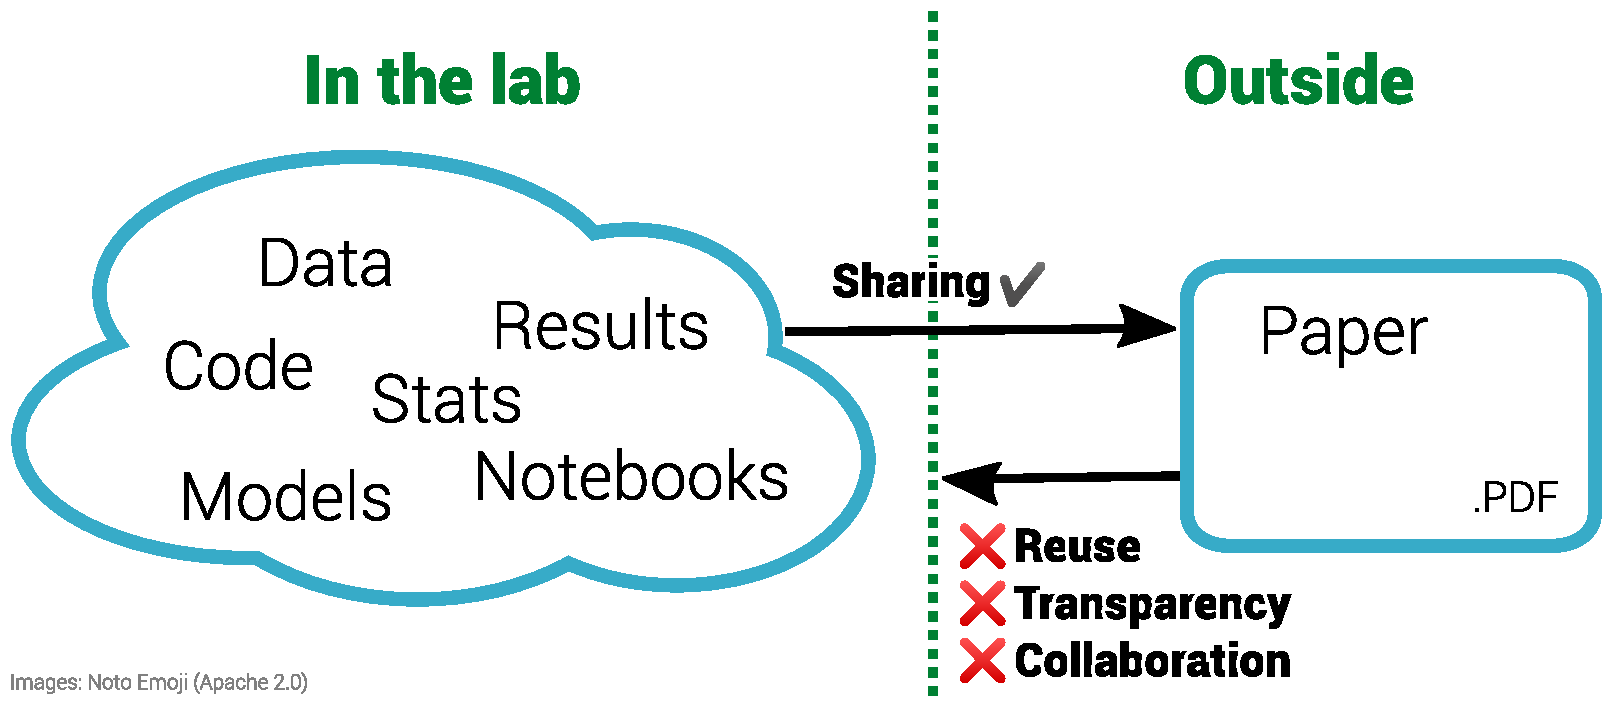
\includegraphics[width=0.7\textwidth]{figs/rr.pdf}
  \caption{The inverse problem in reproducible research.  The left
  half of the diagram shows the diverse range of materials used
  within a laboratory.  These materials are often then
  condensed for sharing with the outside world via the
  research paper, a static PDF document.  Working backwards from the
  PDF to the underlying materials is impossible. This prohibits reuse
  and is not only non-transparent for a specific paper, but also 
  ineffective for science as a whole. By sharing the
  materials on the left, others outside the lab can reproduce
  or build on this work.}
  \label{fig:inverse}
\end{figure}

\section*{What is a CODECHECK?}\label{what-is-a-codecheck}

\subsection*{Workflow and people}\label{workflow-people}

CODECHECK is best demonstrated by way of our example workflow, and later
we expand on the underlying principles. The workflow involves three
groups of people: (1) the AUTHOR of a paper providing the code to be checked, (2)
the PUBLISHER of a journal interested in publishing the paper by the
AUTHOR and (3) the CODECHECKER who checks that the AUTHOR's code works.
The workflow that we have refined is documented in Figure~\ref{fig:workflow}.

% TODO: how is a CODECHECK different from a "specialist reviewer" ? Is it because it is not special, but regular?

\begin{figure}
% original figure source: https://docs.google.com/drawings/d/1tGOZFNZle-oE1Ynw_tLZFmNcv3wgxD0HPs5bXzDOrng/edit
% emojis: https://github.com/googlefonts/noto-emoji and https://github.com/twitter/twemoji
% emoji codes:
% book stack: 1f4da
% package: 1f4e6
% file drawer: 1f5c4
% disk: 1f4be
% document: 1f4c4
% phd: 1f393
% detective: u1f575
% laptop: 1f4bb
% folder: 1f4c1 1f4c2
% receipt: 1f9fe
  \centering
      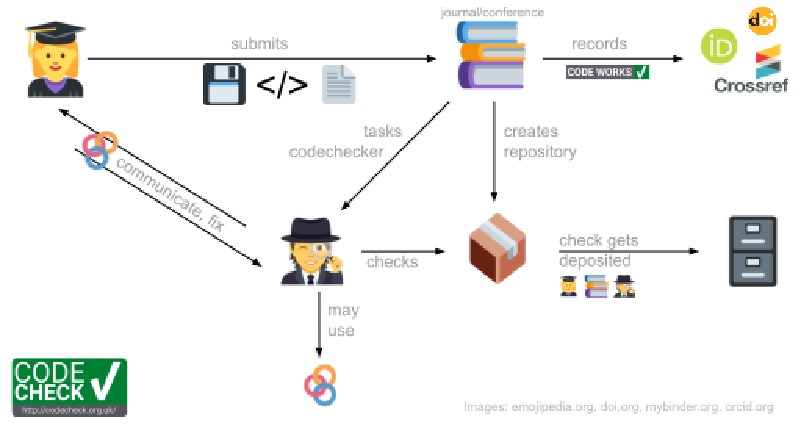
\includegraphics[width=\textwidth]{figs/codecheck_overview.pdf}
  \caption{The CODECHECK example process implementation. Codechecker act as a detectives:
  They investigate and record, but do not fix issues.}
  \label{fig:workflow}
\end{figure}

\textbf{Step 1:} the AUTHOR submit their manuscript along with code and data to
the PUBLISHER. The code and data need not be openly available at this point.
However, in many cases the code and data may be published on a code hosting platform,
such as GitHub or GitLab. Ideally, the AUTHOR is expecting the CODECHECK and
prepares for it, e.g., by asking a colleague to briefly attempt a reproduction
of the submitted workflow.

\textbf{Step 2:} the publisher finds a CODECHECKER to check the code. This is
analogous to the publisher finding one or more reviewers to evaluating
the paper. However, a crucial difference is that we suggest the CODECHECKER
and the author can talk freely to each other directly (see next).

\textbf{Step 3:} the CODECHECKER runs the code, based on instructions provided by
the author, and checks if some/all of the results from the paper can be
reproduced. (See later for exact nature of ``reproduced''). If there are
any problems running the code, the CODECHECKER asks the AUTHOR for help
to resolve the problems. The burden to provide reproducible material lies with
the author.
The CODECHECKER then tries to run the code again.
This process iterates until either the CODECHECKER is successful,
or the CODECHECKER concludes the code does not work (\emph{TODO NOT
  YET HANDLED}). As part of this process, the CODECHECKER could work entirely
locally on their own compute resource, or in the cloud, e.g.~using the open
MyBinder infrastructure \cite{jupyter_binder_2018} or alternatives, some of which
are more tailored for scientific publications while others offer commercial
options to, e.g., publishers (cf. \cite{konkol_publishing_2020}).
Using such cloud-based 
infrastructure allows for the CODECHECKER and author to collaboratively improve
the code and enforces a much more complete definition of the computing environment,
but, unless secure infrastructure is provided by, e.g., by the publisher, requires code
and data to be published openly online.
Note that the task of the CODECHECKER is to check the ``mechanics'' of the
workflow, not to evaluate its correctness. 
Stodden et~al. \cite{stodden_setting_2013} distinguish between verification and
validation in the context of Mathematics, and in the same vein a CODECHECK
ensures a verification\footnote{Note this is a different use as the \emph{Verification Reports} article type in the journal \emph{Cortex}
\cite{chambers_verification_2020}},
i.e., checking that the code correctly produces the 
output it claims to create, but not a validation, i.e., does the code implement
the right algorithm to solve the problem that is researched, 
of the computational results.
Nevertheless, the simple attempt to reproduce may highlight shortcomings in
a submission with respect to transparency as it may be required by a journal's
policy and help to resolve misunderstandings and discrepancies
(cf.~\cite{christian_journal_2020}).

\textbf{Step 4:} the CODECHECKER writes a certificate stating how the code was
run and includes a copy of outputs (figures, tables) that were
independently generated. The certificate may include further recommendations to
the author how to improve the material.
The plain text in the certificate is the most flexible and feasible way to 
make clear what was really checked. Readers will have very different 
understandings of what a ``green'' checkmark (cf. Step~5) means.

\textbf{Step 5:} the certificate as well as auxiliary files created
during the check, e.g., a specification of a computing environment,
helper scripts, and the code and data, if available under open
licenses, get deposited in an open archive (currently Zenodo); the
certificate is given to the PUBLISHER.

\textbf{Step 6:} the PUBLISHER can then use the certificate as part of their
supplementary records for a paper or provide it to scientific reviewers; the
PUBLISHER also gives credit to the CODECHECKER for their work by depositing the
activity appropriately in scholarly publication databases, such as ORCID.
The PUBLISHER also ensures proper publication metadata, e.g., links from the 
certificate repository to the published paper or the original code repository.
A badge or other visual aid may be applied to highlight the fact of a completed
CODECHECK and provide a incentive and reward for the, today often considered
``additional'' efforts of providing readily computationally reproducible workflows,
despite the simplification into a binary value and the possible confusion of
the meaning, especially across disciplines and methods.

\subsection*{Variations}\label{variations}

\subsubsection*{Dimensions of CODECHECK workflows}\label{dimensions-of-workflows}

The example workflow leaves room for different
implementations of this process. To elaborate on these options, we consider
the following dimensions in a space of possible CODECHECK workflows, as shown in 
Figure~\ref{fig:dimensions}, to represent relevant aspects for the involved
stakeholders. These aspects touch on timing, responsibilities, and 
transparency and will be discussed in the following sections.
Each of these have their own pros and cons and can for the most part be
freely combined.

\begin{figure}
% original figure source: https://docs.google.com/drawings/d/1q2EdW3Ad-IpcD-CeoR1eIFMJW2fF6OVmDhCtCUmLO1k/edit
  \centering
      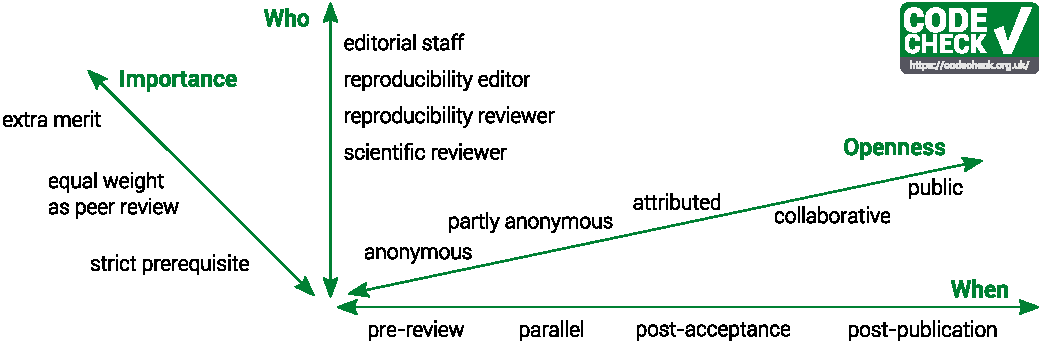
\includegraphics[width=0.8\textwidth]{figs/codecheck_dimensions.pdf}
  \caption{The dimensions of implementing a CODECHECK process.}
  \label{fig:dimensions}
\end{figure}

\subsubsection*{When to do a CODECHECK and with what importance?}
\label{when-to-do-a-codecheck}

The point in time when a CODECHECK happens greatly depends on the 
intentions and the ascribed importance.
The earlier a CODECHECK happens in the process, the more the
results can play a role in editorial decisions:
is a paper published, sent back for revisions, or rejected.
Such a \textbf{strict prerequisite} can reduce the workload of reviewers,
and therefore seems out of place late in the review process.
The later in a review process the check happens, the less challenging is it
to allow a bidirectional communication between author and codechecker, e.g.,
because the author might already be notified of the acceptance and may more
freely share materials online.
Even earlier checks, i.e., a CODECHECK of a preprint, may even help to 
improve the workflow itself even before a publisher is involved. The 
possibility for codechecking papers could be part of a preprint server's
policy, or simply be initiated by interested readers and community members.
% TODO add a sentence about the possible effect of just asking for
% code/data early on in the submission process, see https://twitter.com/tsuyomiyakawa/status/1230672758163402752?s=09)

We see a CODECHECK as part of a typical scholarly communication process.
While more radical ideas to change the paradigms
how researchers share their work exist\footnote{For example Octopus, 
\url{https://science-octopus.org/about}, or Hypergraph
\url{https://www.libscie.org/hypergraph}.},
% mimosa is another platform idea, but no real prototype AFAICT:
% https://projects.invisionapp.com/share/E9Z3RKE7W3P#/screens/436978924
% https://docs.google.com/presentation/d/1V_K8hghgnvGfEtW7TdwtowTveZyy4Qs8rMemNyHx_Dg/edit#slide=id.p
there is a value in an evolutionary approach.
Thereby, existing communities can 
transition towards more open practices at their own pace and ensure
no one is left behind unfairly.
When integrating a CODECHECK in existing review and publication processes,
the \emph{turnaround time} is crucial. Depending on when and who conducts
the check, it may be done faster, or add considerably to the overall
time from submission to publication.
In our first checks, we found that a codecheck may generally take from 2-5
hours, with some outliers on the higher end. This time includes writing and
publishing the certificate, but excludes the time for actual computations.
These efforts include considerable time to communicate about the process, 
especially around who publishes which document when, so that proper 
cross-referencing between paper and certificate is ensured via persistent
identifiers.
When integrated into a peer review system, this handling of documents should
become much more effective and reduce organisational efforts.

A \textbf{pre-review} CODECHECK allows editors to use it as a filter to only
send  a submission out to peer review if it passes the check.
The certificate would  be included in the submission package provided
to the reviewers, so they can include the CODECHECK's results in their 
evaluation of the work.
Reviewers may then judge the the relevance of the computations for the results
of the work, or follow journal guidelines as how strict to apply the check's
outcomes.

A CODECHECK may also be conducted in \textbf{parallel} to the scientific review.
This puts less burden on the turnaround time for the check, yet only makes the 
outcomes available for the final consideration of the handling editor.
The check could also be tasked on demand, e.g., only if one of the reviewers
suggests/requests one because previous screenings might not have caught the 
fact that a computational workflow is part of the submission. However, 
soliciting such a "specialist review" is much more undesirable than having
a regular CODECHECK, without any special treatment for some submissions.
A CODECHECK could then be awarded \textbf{equal weight} as the other reviews.

A \textbf{post acceptance} CODECHECK puts the least requirements on the author 
and may simply lead to an award of excellence on top of the acceptance of the
submission. This \textbf{extra merit} is the least strict solution while still
properly  acknowledging the check results,
because the CODECHECK is to be completed 
before the publication of the final paper.
The GIScience group of checks (see \nameref{register}) falls into this
category: the AGILE conference highlights articles where the reproducibility
was successfully reviewed with a badge on the volume and article landing
pages. Similarly, the GIScience papers in collaborations with journals were 
checked while the authors worked on revisions.

Finally, a CODECHECK may also be conducted \textbf{post publication}, though it
would required to update the article and article metadata later to reference 
the check, otherwise readers would presumably not be aware of it. In general,
publishers are hesitant to make such a revision of published articles.
While this has the least impact on the current publishing practices and also
enables open discourse,
it also has the smallest effect on the original submission
and does not acknowledge the importance of reproducible workflows for
ensuring good scientific practice.

\subsubsection*{Openness, or: Who knows who?}\label{who-knows-who}

The topic of blinding is broadly discussed, not the least in the push towards
open peer review as part of the Open Science movement 
(cf. \cite{ross-hellauer_guidelines_2019}).
Without taking a strong stance on this discussion, the general motivation 
for more  transparency and reproducibility does indeed favour a more open 
review process.
However, anonymity can also serve to protect individuals 
\cite{tennant_limitations_2020}, e.g.,  junior scientists, whereas it might 
be acceptable to require revealing of the names of tenured researchers.
The possible negative effects of a non-anonymous review are greatly reduced
if a CODECHECK is not relevant for the decision to accept or reject, but that
is of course not desirable. Instead, we argue that a CODECHECK is technical
process that should in any case be fixable and not a question of opinion or
faulty approach. It is technically possible for a nonsense workflow to receive
a CODECHECK certificate.
If passing a CODECHECK becomes mandatory, the full transparency may have to be 
revisited as the relations between authors and codecheckers fall under the
same social and acommunity challenges as non-anonymous peer review
(cf.~\cite{everythinghertz123}).
% previous sentenc inspired by https://osf.io/9cftx/
Furthermore, the level of documentation that is needed for third parties
to reproduce a workflow is extremely hard to get right. Too often, this 
uncertainty leads to researchers giving up and not documenting at all.

The technical nature of the check and the challenge of good enough 
documentation is why we see great benefits in a effective bidirectional
means of communication between author and codechecker. Instead of trying to
fix problems or guess the next step, the codechecker can ask the author to 
rework the docs  or the code.
Instead of lengthily describing a small change, the codechecker may simply
provide a fix within the code.
Instead of hiding useful and  instructive files created during the codecheck
(e.g., a machine-readable computing environment specification), the author 
and readers can profit from the software-related expertise of the
codechecker.
While such a communication may be facilitated in an anonymous way by the 
publisher, it most likely only helps to protect the identity of the 
codechecker, because, especially when of a certain size, not trivial, or 
if very specialised, it is close to impossible to fully anonymise a 
software analysis stack.
Therefore, the most effective means with the most desirable result for
the stakeholders is a non-anonymous and collaborative CODECHECK.
The possible contributions by the codechecker may even be integrated into
the code of the workflow and be acknowledged as code commits. This way, 
proper credit is given within the research software development community.
Nevertheless, depending on other needs represented by other dimensions,
the aspect of `Who knows who?' may be the most flexible one.

\subsubsection*{Who does the CODECHECK?}\label{who-does-the-codecheck}

The options for the person who can conduct a CODECHECK require a not quite
simple matching of a combination of skills and availability. Ideally, the
codechecker has a matching code \emph{and} domain expertise, for example to
check a workflow based on Python code analysing neuroimaging datasets. However,
a well-documented workflow should be executable by any person with a basic
understanding of computers. Naturally, the more prerequisite knowledge the
codechecker has, the less time is needed to understand the goals and 
the mechanics of an analysis. From our experiences, the priority should be
given to matching technical expertise first, as the a lack of knowledge in
setting  up a computing environment with a particular language or tool is 
much more discouraging and the assessment of the outcome, e.g., comparing
created figures with the original, is largely possible without 
understanding the science.
The time and expertise allotted to the check
are the main drivers for the depth of checking, though in general, we 
expect a CODECHECK not to evaluate performance, e.g., does a racing car
have the best apex speed, but to assess operation free of failure, i.e., 
is it a car with 4 wheels and at least one door, and does it move forwards
when accelerating. This depth can be seen independent from the power of
the check (see above), as long as it is communicated clearly to all
stakeholders, most importantly authors and readers.

The concrete people to provide these expertises can range from researchers,
possibly drawn from the regular pool of volunteer
\textbf{scientific reviewers} or from a special group of
\textbf{reproducibility reviewers}, via specific roles
such as \textbf{reproducibility editors}, to experts working as part of
\textbf{editorial staff} with a publisher. If the regular reviewers
are relied upon, the editor's task to find suitable ones becomes more
tedious; extra information such as software familiarity would have to be
modelled in review platforms.

We consider a \emph{single codechecker} to be enough, unlike peer review where
multiple referees are common. Because of the technical focus, the 
determination if the concrete outputs of author and codechecker, who can
collaborate to solve any issues, actually match should be a very factual 
process and not
require much debate or opinion. Code usually makes systematic and repeatable
mistakes is is thereby more reliable and auditable than processes controlled
by humans \cite{tibav:42484}, e.g., in a laboratory.

Depending on the importance of the CODECHECK
(see \ref{when-to-do-a-codecheck}), a mediator, e.g., the editor, or a
second opinion might be warranted in rare cases.

We see a great opportunity to especially involve
\emph{early-career researchers}
(ECRs) as codecheckers. They arguably have a high interest in learning
about the latest tools and technologies as they are building up their own
expertise and specialisation. The possibility to gain insights into latest
science for ECRs and at the same time increase the appreciation of
reproduction efforts is a sweet spot that CODECHECK shares
with \emph{ReScience X}, a journal devoted to reproduction and replication 
experiments \cite{roesch_new_2020}.
In fact, ECRs are often much more familiar with latest technology and are 
likely to be early adopters as creators, i.e., be authors of CODECHECK-ready manuscripts, too\footnote{Cf. the 77\% of 141 registered reports who were 
submitted to leading Neuroscience journals by ECRs
\cite{chambers_registered_2019}.}
They are also introduced to peer review and 
may transition into the role of scientific reviewer over time.
Not to solve the general problems of peer review, which is largely an
unsupervised process, i.e., rarely are reviewers taught how to do it, but
a junior codechecker may be supported by a senior codechecker, too.
We see a high potential in setting up the new processes for CODECHECKING with
a clear commitment on openness and transparency, independent of the
respective current peer review process (see \nameref{who-knows-who}).

A publisher's \textbf{editorial staff} represents the most controlled but also
resource-intensive
option. Hiring the required technical and or domain expertise puts a financial
burden on the publisher, of course, but such a commitment also shows the 
value given to publishing reproducibility and would positively impact the 
submission experience, because of more controllability, and external 
perception of the journal or conference. A staff codechecker reduces the 
challenges when it comes to open communication and awarding credit, as
in-house personnel may be more readily be given access to non-anonymised
submission material and receives a proper salary instead of public credit
as part of the scientific community.
Keeping diverse specialists as staff to realise a codechecking process is 
unlikely to be feasible, especially for small or independent publishers.

In contrast, for researchers it can be very important to be publicly credited
with their activity as a reviewer (see TODO CHECK REF \nameref{who-knows-who}).
A regular
review may be listed in public databases (e.g., ORCID
\footnote{\href{https://support.orcid.org/hc/en-us/articles/360006971333-Peer-Review}{https://support.orcid.org/hc/en-us/articles/360006971333-Peer-Review}} or commercial offerings such as Publons
\footnote{\href{https://publons.com/}{https://publons.com/}} or 
ReviewerCredits\footnote{\href{https://www.reviewercredits.com/}{https://www.reviewercredits.com/}}).
A codechecker should be listed just the same. The number of scientific reviews
is of course a very coarse indicator for the community contribution by an 
individual, yet it is unclear if a regular reviewer, who in addition
conducts a CODECHECK to the scientific review, should be credited twice.

The codecheckers community\footnote{\href{https://github.com/codecheckers/codecheckers/}{https://github.com/codecheckers/codecheckers/}}
currently has over 20 individuals who signed up as volunteer codecheckers
following talks given on the project in the last 12 months.
That is even though no checks are actively elicited.
We see a high potential in an open shared list of potential codecheckers 
compared to a private, in-house group, as it may better match expertise
and share the workload.
% TODO tell more about the motivations and commitments that we know about?
The overarching community is also a mean to ensure CODECHECK is a viable
option not just for large publishers, independent of their financial model,
but also for independent no-cost open access journals.

\section*{Core principles}\label{core-principles}

The example workflow and variations just outlined above reflect our current
views on how a codecheck should be performed. They are not set in
stone, but we do believe the following core principles underpin our
CODECHECK:

\textbf{1. Codecheckers record but don't investigate or fix.} The
codechecker follows the instructions provided by the author in running
the code. If any steps are unclear, or if code does not run correctly,
the codechecker records this fact, and then communicates this
information to the author. We believe that the job of the codechecker is
not to fix all these problems, but simply to report them, and await a
fix from the author.

\textbf{2. Communication between humans is key.} Some code may just
work without any interaction (e.g. CODECHECK certificate 2020-013
\cite{cert-2020-013}); however, more often there are hidden
dependencies that need to be found, or revised software
installations. Allowing the codechecker and human to communicate
directly and openly with each other should make this process as
constructive as possible. We feel that routing this conversation
(possibly anonymously) through a publisher would slow things down and
reduce the chances for community building as well as the lessons
learned for both author and codecheckers.

\textbf{3. Credit is given to codecheckers.} The value of contributing a
CODECHECK is comparable to providing a scientific peer review. Individual
variations aside, it may also require a similar amount of time. Therefore,
the codechecker's activity should be publicly recorded and mentioned in the
published paper.
The public record can be realised by publishing the certificate in a 
citable form (i.e., with a DOI; this is done within the community codecheck
process), by listing codecheckers on the journal's website or, ideally, by
publishing the checks alongside peer review activities in public databases.

\textbf{4. Workflows must be auditable.}
This requires that the codechecker 
has at least enough material to validate the workflow outputs submitted by 
the authors. Stark~\cite{stark_before_2018} calls this `preproducibility'
and the ICERM report \cite{stodden_setting_2013} defines the level
``Auditable Research''  similarly.
Every community may establish their own good practices or adapt generic
concepts and practical tools, such as publishing all building blocks
of science in a research compendium
\footnote{\url{https://research-compendium.science/}}.
A completed check means that code could be executed at least once without
critical errors or
warnings using the provided instructions, and, therefore, all code and data 
was given and could be investigated more deeply or extended in the future.
Ideally, this is a "one~click" step, but achieving this requires particular 
skills. It is also hard to create a sufficient level of documentation for 
third parties. Furthermore automation may lead to people gaming the system
or reliance on technology hiding important details. All such aspects can
reduce the understandability of the material, which we estimate to be the
best mean to ensure long-term transparency and usefulness.
That is why the possibility to communicate is more important
than perfected workflows, and why a CODECHECK is not automated.
We acknowledge that others have argued in favour of bitwise reproducibility
because in the long run it can be automated\footnote{Konrad Hinsen on 
Twitter: \url{https://twitter.com/khinsen/status/1242842759733665799}};
but until then we need CODECHECK's approach.

\textbf{5. Open by default and transitional by disposition.} % or "design"?
By default, unless there are strong
reasons to the contrary (e.g., clinically-sensitive data), all code and
data, both from author and codechecker, will be made freely available, i.e., 
under open licenses, before or when the certificate is published.
Note that openness is not required for the paper itself as to accommodate 
journals to transition to sustainable open access models.
The code and data publication should follow community good practices.
By disposition, a CODECHECK workflow should be designed (a) as a recognition of
shortcomings in asserting reproducibility of submissions and (b)
with an understanding of the
complex situation that lead to this. However, establishing a CODECHECK workflow
should go hand in hand with initiatives and a perspective to improve education
around reproducibility of methods and communication of comprehensive 
computational workflows, with the long term goal for a specific community or
journal's target audience to reach a state where the level of verification 
and trust provided by codecheckers becomes part of peer review and regular
merit of all accepted papers.

\section*{Implementation}\label{implementation}

\subsection*{Register}\label{register}

We have a curated list of 25 certificates available at
\url{https://codecheck.org.uk/register}. These are a mixture of
reproductions of papers for a variety of reasons and fall into three themes:
(1) classic and current papers from computational neuroscience,
(2) COVID-19 modelling preprints, and
(3) GIScience.  
The first theme was the initial set of papers used to explore the concept
of CODECHECK. The idea was to take very well known historical articles from a 
specific domain, in this case the work area of co-author SJE, possibly 
as as a conversation starter for potential collaborating journals.
The second theme is rather opportunistic. As the COVID-19 pandemic swept
over the whole Earth, we hoped to contribute a small part to science's answer
to the unknown virus. The checks were solicited through community interaction
%Several COVID-19 models have been done during the time of peer review of these papers,
and under our initiative rather than requested from journal, but the certificate
has then been acknowledged/cited in the paper \cite{Davies2020-vj}.
The third theme represents co-author DN's service as Reproducibility
Reviewer at the AGILE conference series.
Independent of CODECHECK, the \emph{Reproducible AGILE} Initiative \cite{reproducible_agile}
established a process for reproducing workflows at the AGILE conference
series \cite{nust_improving_2020}.
While using slightly different terms and infrastructure, e.g., ``reproducibility
reports'' are published on OSF instead of certificates on Zenodo, the 
reproducibility reviews adhere to the codecheck principles.
Furthermore, a small number of checks was completed as part of a peer reviews
for GIScience journals.

Table~\ref{tab:register} lists the certificates completed to date,
along with citations to the original papers.
Out of these areas, we would like to briefly highlight three examples here.

\textbf{TODO: SJE, tidy this paragraph.}
\begin{enumerate}
\def\labelenumi{\arabic{enumi}.}
\item
  Gigascience -- our first paper.  Only visualisation, not machine
  learning (which would have taken several days of compute time).
\item
  report 9 -- covid model of UK lockdown model -- unlike many claims
  in the popular media at the time, the model was reproducible
  [NOORDEN news piece]. 
\item
  Manuel's certificate -- approached us as he requested a certificate
  as paper was entering peer review.
\end{enumerate}

\begin{table}
  \footnotesize

  \centering

  \begin{tabular}{llp{12cm}}
    \toprule
    \textbf{Certificate} & \textbf{Research area} & \textbf{Description} \\ \midrule
    2020-001 \cite{cert-2020-001} & Machine learning & Code for benchmarking ML classification tool checked post acceptance of manuscript and before its publication in \textit{Gigascience} \cite{Piccolo2020-lo}. \\
    2020-002  \cite{cert-2020-002} & Neuroscience & Code written for this project checked by second project member as demonstration using paper from 1997 showing unsupervised learning from natural images \cite{Hancock1992-mp}. \\
    2020-003  \cite{cert-2020-003} & Neuroscience &  Code written for this project checked by second project member as demonstration using classic paper on models of associative memory \cite{Hopfield1982-mz}. \\
    2020-004  \cite{cert-2020-004} & Neuroscience & Code written for this project checked by second project member as demonstration using classic paper on cart-pole balancing problem \cite{Barto1983-rg}. \\
    2020-005  \cite{cert-2020-005} & Neuroscience & Check of independent reimplementation of spike-timing-dependent plasticity (STDP) model \cite{larisch_re_2019} conducted as demonstration for this paper. \\ % Python ANNarchy
    2020-006  \cite{cert-2020-006} & Neuroscience & Check of independent reimplementation of a generalized linear integrate-and-fire neural model \cite{detorakis_re_2017} conducted as demonstration for this paper. \\
    2020-007  \cite{cert-2020-007} & Neuroscience & Check of independent reimplementation of analysing spike patterns of neurons \cite{hathway_re_2018} conducted as demonstration for this paper. \\
    2020-008  \cite{cert-2020-008} & COVID-19 & Code for modelling of interventions on COVID-19 cases in the UK checked at preprint stage \cite{davies-preprint-2020} and later published \cite{Davies2020-vj}. \\
    2020-009  \cite{cert-2020-009} & COVID-19 & Code for analysis of effectiveness of measures to reduce transmission of SARS-CoV-2 checked as preprint \cite{kucharski-preprint-2020} and later published \cite{kucharski_effectiveness_2020}. \\ % R, check mentiond in acks, but not linked
    2020-010  \cite{cert-2020-010} & COVID-19 & Code for analysis of non-pharmaceutical interventions (Report 9) checked as a preprint \cite{ferguson_report_2020}. \\ % CovidSim
    2020-011  \cite{cert-2020-011} & COVID-19 & Code for modelling of COVID-19 spread across Europe was provided by authors and checked while paper was in press \cite{flaxman_estimating_2020}. \\
    2020-012  \cite{cert-2020-012} & COVID-19 & Code for modelling of COVID-19 spread across the USA was checked as preprint \cite{unwin_report_2020} and later published \cite{unwin_state-level_2020}. \\
    2020-013  \cite{cert-2020-013} & Neuroscience & Code for analsis of rest-activity patterns in people wihout con-mediated vision was checked as a preprint \cite{Spitschan2020.06.02.129502} after direct contact with the authors. \\ % MATLAB
    2020-014  \cite{cert-2020-014} & Neuroscience & Code for analysis of pertubation patterns of neural activity was checked after publication as part of publisher collaboration \cite{Sadeh2020}. \\ % MATLAB
    2020-015  \cite{cert-2020-015} & Neuroscience & Code for a neural network model for human focal seizures was checked after publication as part of publisher collaboration \cite{Liou2020}. \\ % MATLAB
    2020-016  \cite{cert-2020-016} & GIScience & Code for models demonstrating the Modifiable Aral Unit Problem (MAUP) in spatial data science \cite{Brunsdon2020} was checked during peer review. \\ % R
    2020-017  \cite{cert-2020-017} & GIScience & Code for spatial data handling, analysis, and visualisation using a variety of R packages \cite{Bivand2020} was checked after peer review before publication. \\ % R
    2020-018  \cite{cert-2020-018} & GIScience & AGILE conference reproducibility report using a demonstration data subset with cellular automaton for modeling dynamic phenomena \cite{Hojati2020}. \\ % R
    2020-019  \cite{cert-2020-019} & GIScience & AGILE conference reproducibility report with subsampled dataset for reachability analysis of suburban transportation using shared cars \cite{Illium2020}. \\
    2020-020  \cite{cert-2020-020} & GIScience & AGILE conference reproducibility report using a container for checking in-database windows operators for processing spatio-temporal data \cite{Werner2020}. \\ % Python + PostGIS
    2020-021  \cite{cert-2020-021} & GIScience & AGILE conference reproducibility report checking code for comparing supervised machine learning models for spatial nominal entity recognition \cite{Medad2020}. \\ % Python
    2020-022  \cite{cert-2020-022} & GIScience & AGILE conference reproducibility report checking code for visualising text analysis on intents and concepts from geo-analytic questions \cite{Xu2020}. \\ % Python
    2020-023  \cite{cert-2020-023} & GIScience & AGILE conference reproducibility report on analysis of spatial footprints of geo-tagged extreme weather events from social media \cite{Owuor2020}. \\
    2020-024  \cite{cert-2020-024} & Neuroscience & Code for multi-agent system for concept drift detection in electromyography \cite{vieira_driftage_2020} was checked during peer review. \\ % R
    2020-025  \cite{cert-2020-025} & GIScience & Adaptation and application of Local Indicators for Categorical Data (LICD) to archaeological data \cite{carrer_application_2021} was checked after peer review before publication. \\ % R
    \\ \bottomrule
  \end{tabular}
  \caption{Register of completed certificates as of October 2020.  An interactive version
  is available at \url{http://codecheck.org.uk/register}. % TODO: SJE to complete...
  }
  \label{tab:register}
\end{table}

\subsection*{Annotated certificate}\label{annotated-certificate}

At the completion of each CODECHECK, a certificate is written that
states which outputs, i.e., numbers, figures and tables, from the 
original article could be reproduced by the codechecker.
This certificate is made openly
available so that all readers of the article can see which elements
have been reproduced.  The certificate also includes links to the code
and data used by the codechecker, allowing others to build on the
work.
The format of the certificates has evolved slightly during the
project, as we have learnt to automate different aspects of the
certification.  

To demonstrate the typical contents of a certificate, in
Figure~\ref{fig:cert} we have annotated the first four out of ten
pages of the certificate \texttt{2020-012} \cite{cert-2020-012}.
The referenced article \cite{unwin_report_2020} describes the modelling COVID-19
across the USA.
%% TODO - has this been published yet?.  No, not yet... in review...
Figure~\ref{fig:cert}A shows the certificate number, and its DOI,
which points to the certificate as archived on Zenodo.
The CODECHECK logo is
attached to the certificate to denote successful reproduction.
Figure~\ref{fig:cert}B provides the key metadata about the check --
which paper was checked, who the authors and the codechecker were,
and when it was checked. Materials
relating to the codecheck are freely available via the Repository
link. This table is generated from machine readable text file, the
CODECHECK configuration file \texttt{codecheck.yml}.
The configuration file collects the core pieces of metadata surrounding
a check and enables current and future automation of workflows and 
meta-analyses.
Figure~\ref{fig:cert}C is a textual summary of how the codecheck was
performed, and any interesting findings.

Figure~\ref{fig:cert}D (page 2 of the certificate) shows a table that
lists the outputs that were generated from the codecheck (this is
termed the MANIFEST).  For each output, there is a comment stating
which figure/table it should be compared to in the original paper,
along with the size of the file.  On page 3 of the certificate,
Figure~\ref{fig:cert}E shows some more detailed notes from the
codechecker, in this case indicating what steps were needed to
initialize the environment and run the code.  This particular example
was quite long, taking about 17 hours to run.  Finally, on page 4 of
the certificate, we see the first output that was generated by the
codecheck (Figure~\ref{fig:cert}F).  In this case, the figure matches
figure~4 of \cite{unwin_report_2020}.
Subsequent pages of the certificate show other outputs (not shown here).

\begin{figure}
  \centering
  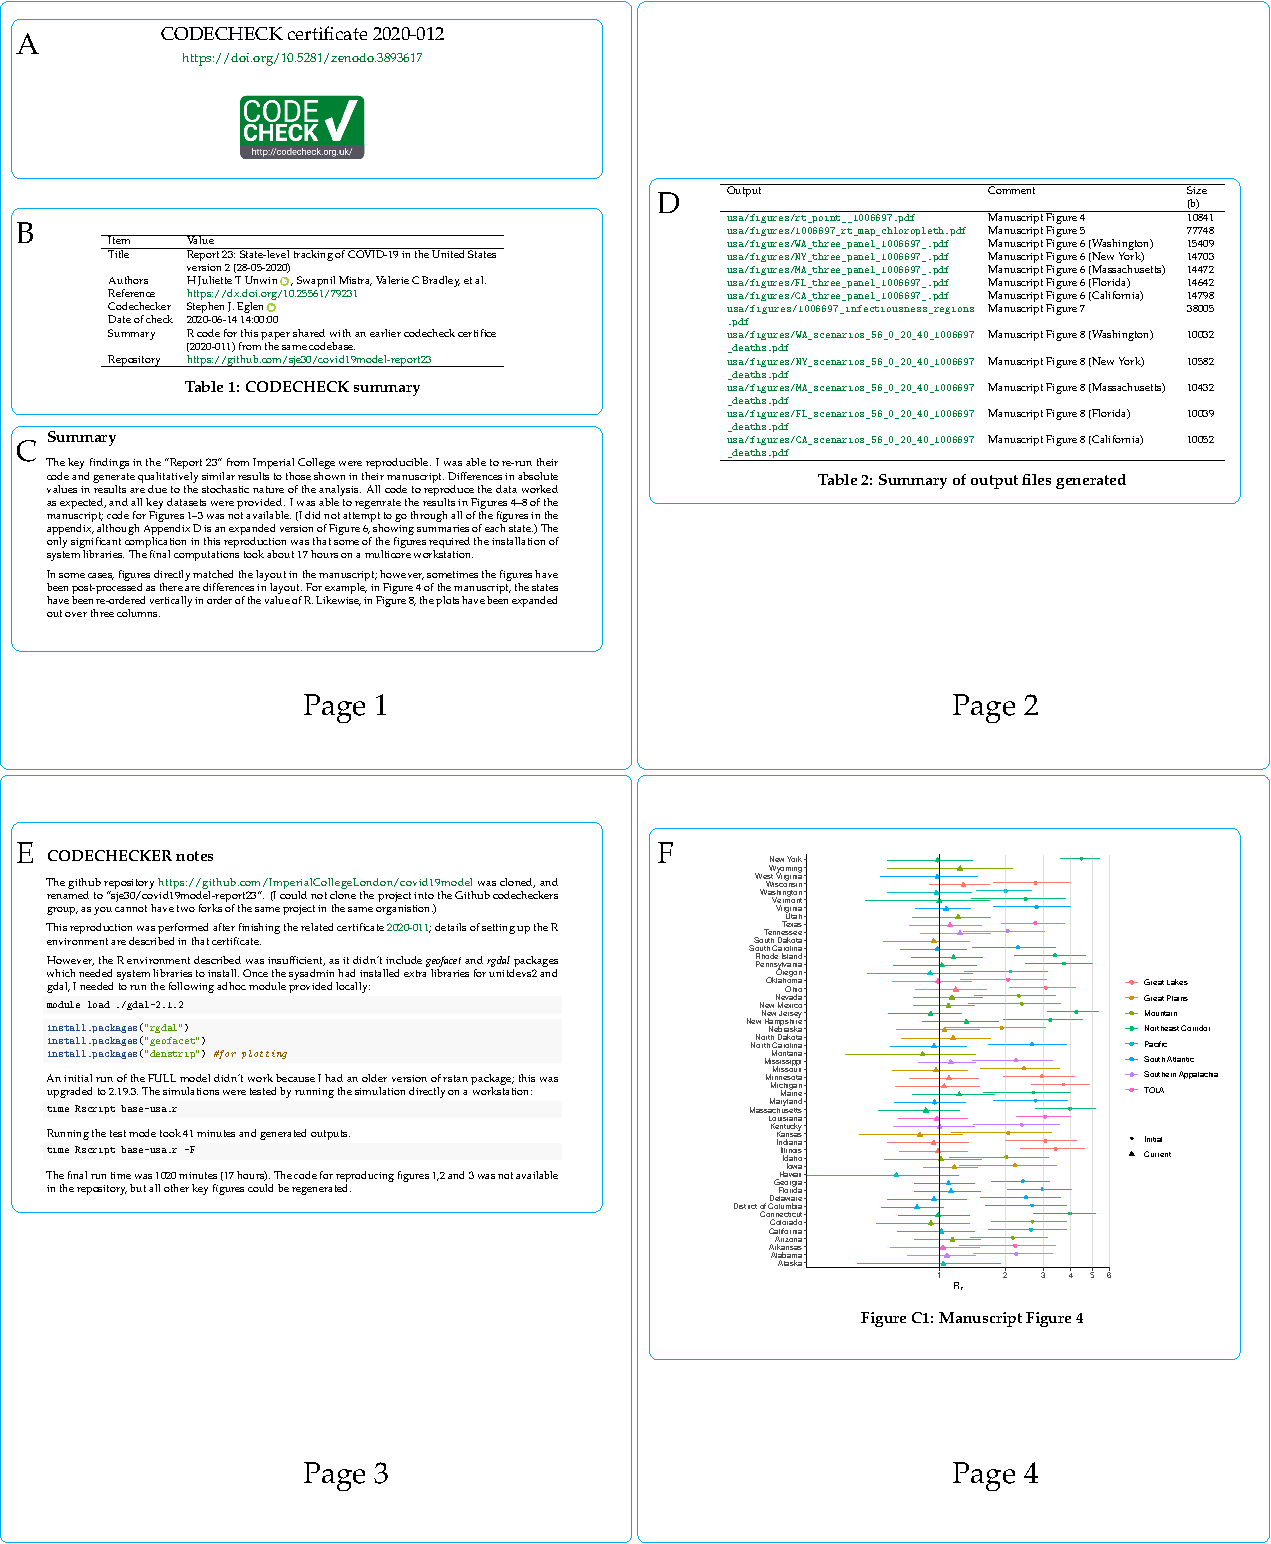
\includegraphics[width=\textwidth]{figs/annotate-cert-crop.pdf}
  \caption{Annotated certificate 2020-012 \cite{cert-2020-012} (first four pages only).}
  \label{fig:cert}
\end{figure}

\subsection*{Tools and resources}\label{tools}

To run the system, we rely on freely available infrastructure, more 
specifically GitHub and Zenodo.

The \texttt{codecheckers} GitHub organisation\footnote{
\url{https://github.com/codecheckers}} contains projects managing the
project website, the community of codecheckers, community discussions,
forks of codechecked code repositories, and the main register for
managing the collection of checks. Both the website\footnote{
\url{https://codecheck.org.uk/}} and the register
\footnote{\url{https://codecheck.org.uk/register}} are hosted as GitHub
pages. The register is effectively a single table in CSV format that
connects the certificate identifier with the repository associated with
a specific conducted codecheck. Each of these repositories, which 
currently can be hosted on GitHub or Open Science Framework (OSF), 
contains the CODECHECK metadata file \texttt{codecheck.yml}. The register
further contains a column for the type of check, e.g., community, journal,
or conference, and the respective GitHub issue where communications and 
assignments around a specific check are organised. No information is 
duplicated between the register and the metadata files. When a new
certificate is entered into the register, an automated process using 
continuous integration infrastructure of GitHub, GitHub Actions, retrieves
the metadata files and builds different representations of the register
for viewing (HTML) or integration with other services (CSV, JSON).

Zenodo is an open repository for scientific data and documents. It
mints DOIs for deposits and ensures long-term availability of all digital
artefacts related to the project. These include the community 
certificates as well as the register, which is regularly archived to 
Zenodo \cite{codecheck_register} (including all file formats).

A custom R package, \texttt{codecheck}\footnote{
\url{https://github.com/codecheckers/codecheck}}, helps with the authoring
of certificates, and with the deposition of certificates and reated files to
Zenodo using the R package \texttt{zen4R} \cite{zen4r}.
Codecheckers may choose to not use the package and rely on their own tools
for creating the certificate. This is a deliberate flexibility to
accomodate both different skill sets and unforseen technical advances or
challenges.

These tools and resources demonstrate that a CODECHECK process can be
managed without infrastructure costs on freely available platforms.
The scripted and automated parts should also ensure that more checks can
be conducted in the future, though the management by a paid CODECHECK
editor or further automation, e.g., with a bot, could improve turnaround time.
The remaining costs are the project's domain, which is negligible, and
the human resources for managing the project and processes, which are
considerable and currently solely based on, partly grant-based, public funding.
Naturally, similar set-ups are possible, such as using GitLab/GitLab.com 
and the GitLab CI instead of GitHub and GitHub Actions, or using a different 
data repository for depositing certificates and data.

\section*{Related work}\label{related-work}

The journal \emph{ACM Transactions on Mathematical Software (TOMS)} 
established a "Replicated Computational Results" (RCR) review process
\cite{heroux_editorial_2015} (using "replicable" with the same meaning 
as CODECHECK uses "reproducible").
The CODECHECK principles were independently developed as we only later 
learned about TOMS RCR, which we judge as fulfilling CODECHECK principles
1 to 4.
Our CODECHECK provides more extensive discussion of the possible variants, 
while TOMS RCR realises one particular workflow for reproducibility 
reviews for one particular journal. \cite{heroux_editorial_2015}
include similar concerns about
selection of reviewers as above. Unlike existing CODECHECK certificates, 
the RCR reports undergo editorial review, but this could very well become
part of CODECHECK workflows at journals.
The publication of the RCR report is seen as a reward for the efforts of
the reproducing person, while the possible conflict of interest of this 
motivation is acknowledged. TOMS also recognises reviewer activity in a 
partnership with Publons
\footnote{\url{https://authors.acm.org/author-services/publons}},
though it is unclear if the author of an RCR report receives both the report
authorship and the reviewer recognition. In any case, this is different
from CODECHECK, which specifically aims at recognition as reviewers.
In our view, this removes the possible conflict of interest while keeping
the public acknowledgement.

Specific to the field of Mathematics, the RCR was also  expected to apply a
review of the software itself if the system it runs on cannot be evaluated by
an independent party.
The TOMS RCR also notes the importance of communication and expects
collaboration between author and RCR reviewers.
The TOMS creators share thoughts around reviewer selection and also put trust
in reviewer judgement over numerical bit-wise perfection.
A key difference is that authors opt-in with an \emph{RCR Review Request} and
the RCR reports, which are very similar to CODECHECK certificates, are
published in the TOMS journal next to the actual papers.
A search on Crossref\footnote{\url{https://search.crossref.org/?q=\%22Replicated+Computations+Results+\%28RCR\%29+Report\%22&from_ui=yes&page=2}; search executed
on 2020-12-10} shows 15 RCR Reports to be published and the workflow to be 
extended to the ACM journal \emph{Transactions on Modeling and Computer 
  Simulation (TOMACS)}
%% SJE TODO - fix footnote
%% \footnote{\url{https://dl.acm.org/journal/tomacs/author-guidelines-%35-rcrini}}.

% 8: https://scholar.google.de/scholar?start=10&q=Replicated+Computations+Results+%22(RCR)+Report%22&hl=de&as_sdt=0,5
% 15: https://search.crossref.org/?q=Replicated+Computations+Results+%22%28RCR%29+Report%22&from_ui=yes&publication=ACM+Transactions+on+Mathematical+Software
% 15: https://academic.microsoft.com/search?q=Replicated%20Computations%20Results%20%22(RCR)%20Report%22&f=&orderBy=0&skip=10&take=10

A number of journals or conferences/workshops provide guidelines for ensuring reproducible publications and their verification.
These include, for example, \ldots{}
% first glimpse into "Code exeuction processes in scholarly publishing" ?
% `https://docs.google.com/document/d/1fMWrFvBTwAYXg5J_bYIjgb-gY7DfQ0DOjx9Vlg_Rbmg/edit# ?
\emph{Information Systems}, with an invited reproducibility paper track
\footnote{\url{https://www.elsevier.com/journals/information-systems/0306-4379/guide-for-authors}}

Another journal initiative is more indirectly connected with reproductions.
\emph{Nature Machine Intelligence} recently introduced a new type of article,
the reusability report \cite{noauthor_research_2020}.
Inspired by the detailed and nuanced submissions to a reproducibility 
challenge, the reusability report focuses on the exploration of robustness
and generalizability of the original paper's claims
\cite{noauthor_research_2020}. This answers the specific community's 
challenges around computational reproducibility and also values these kind
of contributions as independent publications, which goes beyond the goals 
of CODECHECK.

However, no approach besides CODECHECK spans across journals and is
intentionally designed to be picked up and implemented by many different 
journals or events, and to build a community of codecheckers. CODECHECK shares
this interdisciplinary nature with other community initiatives concerned with 
reproducibility awareness, education, and supports, such as ReproHack
\footnote{\url{https://reprohack.github.io/reprohack-hq/}}, Code Copilot
\footnote{\url{https://twitter.com/Code_Copilot}}, or Papers with Code
\footnote{\url{https://paperswithcode.com/about}}.
The latter recently announced a collaborations with the preprint server
\emph{arXiv} on providing data and code supplements for machine learning
manuscripts\footnote{\url{https://medium.com/paperswithcode/papers-with-code-partners-with-arxiv-ecc362883167}} and runs a reproduciblity challenge
\footnote{\url{https://paperswithcode.com/rc2020}}.
% Papers with Code now also does more disciplines than just ML.
Likewise, different disciplines and journals provide reproducibility
checklists, e.g., \cite{rosenberg_next_2020}, which naturally share some
aspects while addressing particularities as well as addressing researchers
from different fields. Regarding the education and guidance for authors, 
we see CODECHECK's role in referencing and linking educational efforts
and helpful material, not as a creator and maintainer of content.

The journal \emph{ReScience C} publishes replications
\footnote{\url{https://rescience.github.io/faq/}};
they do not accept proprietary software and require open source code;
they also required a third party to replicate; they also use Zenodo
to issue DOIs.
The journal \emph{Cortex} has a special article type 
\emph{Verification Reports}, which  actually are about replication of results 
but are very well designed/reasoned \cite{chambers_verification_2020}.
In a similar vein, the CODECHECK certificates
could also be published as a special article type within journals.

For research with very high stakes, where reproduction would be too weak and
post publication replication possibly too late because of policy impact,
\cite{benjamin-chung_internal_2020} propose \emph{internal replication}.
A workflow that underwent internal
replication would very likely be of high quality and relatively easy to codecheck.
In a similar vein, internal codechecks may be used, with the same limitations such
as group think \cite{benjamin-chung_internal_2020},
to ensure reproducibility before submission. The guidelines
for CODECHECK can be used by fellow/not independent lab members just as well.

Gavis and Donoho \cite{gavish_universal_2011} propose a new discipline and 
infrastructure for reproducible computational research with its own tools and
API. Their specific packaging format, provenance record, and cryptographic
\emph{Verifiable Result Identifier} would indeed provide excellent
reproduciblity. However, the system is also complex and was not taken up by
any publisher as far as we know; the system is indeed not open source itself.
In comparison, CODECHECK is less powerful but also much more flexible and
less dependent on specific tools or infrastructure. If data and code are 
deposited properly, i.e., very unlike to disappear, then the certificate's 
DOI is practically quite close to the cryptographic identifier.

Local reproduction initiatives/services:
\href{https://ciser.cornell.edu/research/results-reproduction-r-squared-service/}{CISER R-squared}
(established/permanent),
\href{https://go.wwu.de/r2s2}{WWU R2S2} (pilot only, focused on reproductions),
\href{https://github.com/OxfordCodeReviewNet/forum}{Oxford code review network (OxCRN)}
(community, broader scope), \href{https://isps.yale.edu/research/data/approach}{YARD 
at Yale} with dedicated staff for replications.
For these, the CODECHECK scope, tools, and practical experiences may be
helpful resources.

\emph{SciGen.Report} is a community-run platform to foster communication on
reproducibility\footnote{\url{https://scigen.report/}}. People can report on
fully, particially or un-successful reproductions post publication.

\section*{Limitations}\label{limitations}

\textbf{Isn't CODECHECK what peer review should be doing already?}
That is correct.  However, the general observation is that the
increasing number of researchers, submissions, and reviews to conduct
under the pressure to publish, puts the scholarly publication system
under a lot of strain.  We also see parallels to the terms
`reproducible research' and `open science'. Establishing a CODECHECK
process is largely an acknowledgement that peer reviewing practices
have faltered to adapt to the challenges of digitisation and
computer-based research or data science. The concept of a CODECHECK,
just as the reproducibility of research and the openness of science,
may be of transitional nature. If the activities described here as
being part of a CODECHECK become the norm for scientific reviews and
publications, then the initiative will have succeeded.  However, the
rapidly changing technology used in research leads us to believe that
a separate role of codechecker and the expertise it brings will be
beneficial in the long term.

\textbf{CODECHECK requirements are not demanding enough}:
CODECHECK by design does not require authors to provide (and sustain) an
eternally functional workflow and neither suggests a specific software stack
or practical approaches, such as research compendia
\footnote{\url{https://research-compendium.science/}},
even if they are very valuable.
Creating something that anyone can reproduce has been called a 
fool's errand
\footnote{\url{https://twitter.com/DougBlank/status/1135904909663068165?s=09}}
and we tend to agree.
However, the package of data, code, and documentation
collaboratively created by authors and codecheckers is a snapshot of a 
working analysis that greatly increases the likelihood of a successful 
reproduction and possibility to extensions by third parties, with access
to suitable resources and matching skill set, in the future.
Concrete implementations of CODECHECK workflows, especially for specific
disciplines, may reify much more helpful guidelines for authors how to
create reproducibility packages.
The author-friendly ``low bar'' should not stay low forever, but cultural
change takes time and the encouragement and guidance that CODECHECK,
as part of the widely accepted peer review concept, can provide may
eventually allow to raise the bar as high as possible, e.g., with
executable research compendia \cite{nust_opening_2017}
or continuous analysis \cite{beaulieu-jones_reproducibility_2017-1}.
However, considering that missing artefacts and lack of documentation
have repeatedly been identified as main barriers to reproducibility
(e.g., \cite{stagge_assessing_2019,nust_improving_2020}),
we would not underestimate the power of a simple check.

It should be noted that a codechecker is not taking the same roles as the
\emph{statistical reviewer}, as it is practices by some journals in the 
biomedical domain (cf.~\cite{petrovecki_role_2009,greenwood_how_2015}).
The statistical reviewer actually evaluates the appropriateness of
statistical methods \cite{greenwood_how_2015} and can support topical
reviewers if, e.g., complex methods or sophisticated variants of statistical
tests are applied \cite{petrovecki_role_2009}.
The codechecker may go equally deep into the review, if they have, by 
intention of by chance, the required expertise and the required time, 
but they are by no means expected to be able to provide
such a level of scrutiny. We can imagine a tiered workflow where the 
codechecker, just as the conventional reviewer, could recommend a detailed
statistical review to the editor as they might come across upon different
hints.
%The CODECHECK provides a certain level of safety with regard to the inherent
%problems that a computational workflow might have. We want to capture the
%obvious errors, but ... https://www.quora.com/What-is-the-difference-between-safety-and-security

An important distinction is that a codechecker does not conduct a 
\emph{code review}. Code reviews are without doubt extremely valuable in 
terms of improving reproducibility and re-usability, and their proponents 
even believe they can improve the science \cite{petre_code_2014}.
Code reviews, however, have quite different structural challenges and 
require even more resources. That said, a well-reviewed codebase is likely
to be easier to codecheck, and the awareness for high-quality code raised
through CODECHECK may lead to more support for code reviewing.
Initiatives and journals that conduct software reviews independently of 
a specific publication or workflow include
ROpenSci\footnote{\url{https://ropensci.org/}},
PyOpenSci\footnote{\url{https://www.pyopensci.org/}},
and JOSS\footnote{\url{https://joss.theoj.org/}}.

Furthermore, the codechecker's task list is intentionally not
overloaded with related concerns, even though they are very important,
such as ensuring proper citation of data and software, or depositing
data and software in suitable repositories. We do expect codecheckers
to be aware of these though and possibly highlight them.

\textbf{Handling failure}: We have no established process for the case
that a reproduction fails. This may be the sign of a pre-selection bias
of the examples, as so far all our codechecks succeeded.
In case of a journal adopting CODECHECK for all submissions, the open 
question remains as what to do in this case will have to be answered.
At the start, we doubt publicly reporting failures (i.e., the code 
would not run) will increase overall reproducibility and recommend not
to share the outcome publicly but to share the latest draft of the 
certificate with the authors.
A negative comment in a CODECHECK certificate or a failed check does
not necessarily mean the paper or the science is bad
(cf. discussion on negative comments in \cite{everythinghertz123}).
Therefore, one must be careful as to the impact of acceptance by authors 
and the concerns of volunteers this approach, or a contrary one, has.
Private feedback for failures and public acknowledgement/encouragement
for successes seems to be the way to go.
% eLife's new model (see https://osf.io/9cftx/) will publish reports evantually, e.g., after preprint has been accepted elsewhere
\cite{Rosenthal2016b} discuss incentives for different actors around the
implementation of reproducibility. We see CODECHECK as one mean for
organisations to invest in reproducibility by creating incentives
until reproducible computations become the norm.

\textbf{Compute time}: for those papers that take significant compute
time (think days, not minutes), who will pay for the compute time?
The openness of CODECHECK certificates could help to establish community
peer pressure, as submitting authors can be evaluated on their engagement
as codecheckers.
The challenges of computational resources can also quickly be reduced when
authors provide a small sample or a synthetic dataset together with the
expected outputs for this small example, which can equally well demonstrate the 
usefulness and validity of their workflow.

\textbf{Proprietary software}: authors can currently provide code that requires
proprietary software. Given the prevalence of proprietary software in
some disciplines, e.g MATLAB, this seems like a pragmatic choice.
However, it prohibits to benefit from open infrastructure for reproducibility
(cf.~\cite{konkol_publishing_2020,perkel_make_2019})
and requires the codechecker to have access to that software.
Non-open software also considerably hampers reuse, especially by researchers
from the global south. Therefore, allowing proprietary software is a compromise
that each implementation of CODECHECK should critically reconsider.

\textbf{Not possible for my data}: 
Solutions for proprietary and sensitive data exists.
Authors can provide synthetic data (cf. \cite{shannon_opening_2018}), some
data can effectively be redacted \cite{oloughlin_data_2015}, and publishers or
independent entities can provide infrastructure for sharing data and workflows
confidentially \cite{perignon_certify_2019} or with access to derived results
but not raw data \cite{shannon_opening_2018},
i.e., data enclaves \cite{foster_research_2018},
or domains of reproducibility \cite{harris_more_2017})

\textbf{Can't someone cheat?} Yes. We don't check it is correct code or
sound science,
just simply that it runs. This `mechanical' test is indeed a very low bar.
Yet, by having the code and (raw) data openly deposited, interested parties can
then examine the code, and knowing that the code will be open we hope will
be an incentive for authors to share. It will also give the opportunity 
to future researchers, potentially with new methods, to look for errors.
This is a much more effective means to avoid cheating than an arms race
trying to catch the cheater with closed datasets and code. This approach
is comparable to the storing of blood samples in sports to detect
doping in the future (cf. \cite{everythinghertz97}).
Another picture that helped us to define the scope of a CODECHECK is:
the codechecker is the forensic photographer, making sure all the details
are captured so that an investigator may, now or in the future, scrutinize
them.

\textbf{Who's got time for more peer review?} Agree.
Ignoring the complex community contract behind volunteered peer review,
the time spent with CODECHECKs likely reduces the individual's time to work
as a reviewer.
However, there are differences to peer review.
First, the technical nature of a CODECHECK can provide a more 
clearly defined scope and expectations compared to conventional 
peer review. The authors are told what to provide and the codechecker
can be told when to stop, for example.
Second, the specific skill set allows to introduce different groups
into the peer review process. ECRs might be attracted to working with
groups to learn more about recent methods and reproducibility practices.
Research software experts (Research Software Engineers, RSE) who might
not regularly be involved in writing or reviewing papers could be 
interested to increase their connection with scholarly practices.
An extra codechecker may simplify the matchmaking an editor has to do
when identifying suitable reviewers for a submission, as technical and
topical expertise can be provided by different people, who must not even
be traditional peer reviewers. In fact, the codechecker could even be
a software professional employed by a publisher.
Third, recall that we expect CODECHECKs to be not anonymous and always
publicly deposited, which is common practice for some journals, but not
broadly practiced. The possibility to ask for clarification or more 
material/information can greatly reduce the digging required and thereby
the time spend.
We also found that the focus on the mechanics of a
workflow and the ability to interact with the authors can make
reproductions very educational. It's a different role and as such could
be a welcome alternation/diversion for researchers to give back their 
time to the community.
With code and workflows, there also is a good chance that a codechecker's
feedback can have direct impact and lead to improvements of the author's 
work that comes with a rewarding experience or even tangible contributions.
While such impact is also part of idealistic peer review, it is
rather rare beyond paraphrased anonymous acknowledgement.

\textbf{Checking multiple times?} If you check a preprint before peer
review or a submission to a journal with non-public review, it might
need checking again as it is modified during peer review.  This is in
part unavoidable, and as happened to us (e.g., certificate 2020-012
\cite{cert-2020-012} has been revised). This can also be desired, if
the interaction between author, reviewer, and codechecker lead to
improvements.  Since checking the manuscript the second time is likely
to be much less work than the first time, this is largely mitigated by
open and regular communication.  The higher the reproducibility and
automation, the more aspects of a CODECHECK may eventually be
supported by automation, though we believe the human codecheckers
should remain the decision maker.  Automatically detecting if results
are ``the same'' is a question intrinsically linked with each unique
process and quite hard to realise for common outputs, such as plots or
maps.  Nevertheless, continuous integration (CI) infrastructure may
help codecheckers, and, without much further work, use scientific
workflows as detectors for when a piece of software breaks if a
workflow is set up to use the latest versions of tools.

As a principle, we do not require results to be exactly the same for a
codecheck to pass, simply that the code runs and generates the output
files that the author claims. Stochastic simulations mean that often
we cannot get exactly the same, or even the same versions of libraries
can generate outputs that differ by operating system
\cite{Gronenschild2012-pp}.

\begin{itemize}
\item modelDB principle: minimum of one figure should be reproducibe.
  Example certificate 2020-016 (I think) which had only a small subset
  of the possible figures. Still useful and worth sharing.
\end{itemize}

\textbf{Not revolutionary enough?}
CODECHECK's approach is to acknowledge the shortcomings around 
computational reproducibility and iteratively improve within the current
system of scholarly communication through journals.
It remains to be proved if this approach is welcomed broadly and if 
involving the traditional system of publishers helps to push the 
conversation along or not.
We have discussed stronger more drastic rules at length, such as only 
considering diamond Open Access journals, community-led no-fee journals,
or journals with collaborative/open peer review, but eventually decided
against them.
We also have considered to require latest technologial solutions which can
support reproducibility (cf.~\cite{konkol_publishing_2020}), but have 
decided to focus on the human interface and the judgement of an experienced
researchers/developer as a more sustainable approach.
The structurelessness of the required data and software gives the needed
freedom to enable all types of research. It could be complemented by
automated scoring (e.g.,~\cite{menke_rigor_2020}, yet automation and 
metrics bears risks that lead us to put our trust in the codechecker.
Note that the focused nature of the CODECHECK principles allows journals
and publishers to innovate on the financial model and peer review practices
at their own pace.

\section*{Conclusions and future work}\label{future-work-and-conclusions}

CODECHECK works!
We have created a considerable number of certificates to demonstrate it.
The creation of the certificates and the interactions with authors and
editors not only improved the principles and the workflow, but also
confirmed the approach taken. This result corroborates findings from
similar evaluations of reproducible computational research in journals and
at conferences.
CODECHECKs and can increase trust in scientific results and the set of 
shared principles and name can through recognition value allow researchers
across publication venues to judge the level of scrutiny that results have
faced. CODECHECK requires direct acknowledgement of the contribution to the
scientific community in the role, not indirectly via citations of 
reproductions, and can be a worthwhile educational activity, especially for
ECRs. A technically simple yet far reaching change would be a special type of 
reviewer activity for codechecking in public researcher profiles next to
conventional peer reviews.

Yet, CODECHECK underlies the same limitations as peer review
in general and is closely connected to larger disruptions and challenges
in scholarly communication
\cite{eglen_recent_2018,tennant_ten_2019,fyfe_mission_2019}, 
including the tensions between commercial publishing and reviewer's often
free labour, and a global pandemic jumbling up scientific publishing
and exposing a broader general audience to science, even preliminary 
results \cite{munafo_what_2020}.
Even more, it is clear that establishing CODECHECK-like systems can be 
impeded by and must be seen in connection to much larger issues in 
science, such as broken metrics or malpractices triggered by publication
pressure \cite{piwowar_altmetrics:_2013,nosek_promoting_2015}.
We certainly do not want the binary attribute of "CODECHECK completed"
to become a factor in bibliometric approaches for performance assesments.
% Mittermaier, Peer Review and Bibliometrics: http://hdl.handle.net/2128/22745
While developed for the current "paper"-centric publication process and
being compatible with different styles of peer review, the CODECHECK 
principles would also work well with novel publication paradigms, e.g.,
peer-reviewed computational notebooks \cite{earthcube_new_2020},
iterative and granular communication of scientific outputs,
such as Octopus\footnote{\url{https://science-octopus.org/}}, 
articles with live-code \cite{perkel_pioneering_2019-1}
\footnote{For example, eLife's ERA, see 
\url{https://elifesciences.org/labs/dc5acbde/welcome-to-a-new-era-of-reproducible-publishing}.},
decentralized infrastructure and public reviewer reputation systems
\cite{tenorio-fornes_towards_2019},
and completely new visions for scholarly communication and peer review
\footnote{Cf., for example, \emph{A modern vision for peer review} by 
Amy J. Ko: \url{https://medium.com/bits-and-behavior/a-modern-vision-for-peer-review-d5f73f0fae07}}.
An explicit segmentation of research steps could even make the focus 
of a CODECHECK easier by only checking the ``analysis'' sub-publication.
The discovery of CODECHECKs could be increased by depositing the reports
into public databases of reproductions, such as \emph{SciGen.Report}.
Public researcher profiles, such as ORCID, may consider different
types of reviewer activity to capture the contributions of independent 
code execution to science.
Notably, the discussed limitations are largely self-imposed for easier
acceptance and evolutionary integration, as to not break the current 
system and increase demands over time without leaving practitioners behind. 

If adopted today, a CODECHECK system, even if temporal in a sustainable 
transition towards more open publication and review practices, can contribute
to increased trust in the results of research. Introducing CODECHECK
should be informed by lessons learned from (introducing) open peer review
(OPR) \cite{ross-hellauer_guidelines_2019}.
All our conversations with publishers and editors at some point
touched on the procedural and technical implications of openness, be it 
that OPR is neither applied nor well-known by stakeholders, or that process
management software would not support such open communication.
We would be keen to use the flexibility of the principles and cooperate
on non-public CODECHECKs to learn more about the advantages and yet unclear
specific challenges. Does CODECHECK work better with OPR?
Each rollout of CODECHECK should be accompanied by studies to ensure 
codechecking does not fall into the same gaps as peer review did \cite{tennant_limitations_2020}
and to ensure positive change within the respective peer review system.
More reproducible practices initiated by CODECHECKs could lead
communities/disciplines to reach a state where authors do provide good
enough material and reviewers have acquired broady enough skills that
the latter will generally conduct a CODECHECK-level of checking, and
only in especially sophisticated cases will a specialised codechecker
be included.
The main challenge for us remains to get journals to embrace the
idea behind CODECHECK and realise processes conform to the principles,
whether they use the actual name for it or not.
The CODECHECK badge is, intentionally, not branded beyond the checkmark
and green colour and simply states ``code works''.
This \emph{cultural change}, however, is needed for the valuation of the
efforts that go into proper evaluation of papers.
Multiple adopting journals will also help to answer relevant questions on
the establishing process (What are crucial decisions or pain points? Can
authors retract code/data once a CODECHECK has started?),
what variants of CODECHECKs will be most common, and how open CODECHECKs
may influence the scope and anonymity of conventional review over time.

With the implementation of CODECHECK workflows, the question of training
codecheckers will become relevant. We expect both a mentoring scheme within
the CODECHECK community (experienced codecheckers provide on the job training
or serve as fallback advisors) as well as collaboration with reproducible
research initiatives such as
ReproHack\footnote{\url{https://reprohack.github.io/reprohack-hq/}},
ReproducibiliTea\footnote{\url{https://reproducibilitea.org/}}
\cite{fitzgibbon_brewing_2020},
and Repro4Everyone\footnote{\url{https://repro4everyone.org/}}
\cite{auer_reproducibility_2020},
to be able to grow the pool of codecheckers as needed.
The initial reaction of the scientific community, where up to today over 
twenty people spontaneously signed up as volunteer codecheckers after talks
on the initiative, makes us feel optimistic that the time is right for 
putting scholarly peer review on the path to facilitate sharing and execution
of computer programs and documenting reproducibility of results.

\subsection*{Competing interests}

SJE is on the editorial board at the journal \emph{Scientific Data}.
DN is reproducibility chair at the Association of Geographic
Information Laboratories in Europe's (AGILE) annual conference.

\subsection*{Grant information}

This work was financially supported by the UK Software
Sustainability Institute and a Mozilla Science mini grant.
DN is supported by grant
\href{https://gepris.dfg.de/gepris/projekt/415851837}{PE~1632/17-1}
from the German Research Foundation (DFG).

\subsection*{Acknowledgements}\label{acknowledgements}
%Collaborators and potential collaborators:
% someone from SpringerNature

% question mark indicates we are waiting for person to respond.
We are grateful to the following individuals for discussions regarding
the work presented here: Andy Collings, Melissa Harrison?, Giuliano
Maciocci, Naomi Penfold (eLife), Rebecca Kirk (PLOS Computational Biology), Scott
Edmunds (GigaScience), and Andrew Hufton? (Scientific Data). Iain Davies and
Yuhao (Sebastian) Wang developed code and example certificates.
We thank Antonio P\'{a}ez (Journal of Geographical Systems) for enabling
CODECHECKs, Carlos Granell and Frank Ostermann for contributing
certificates as reproducibility reviewers at the AGILE conference, and 
all authors of auditable workflows for their participation.

\subsection*{Author contributions}

DN and SJE contributed equally to all aspects of this project.

{\small\bibliographystyle{unsrtnat}
\bibliography{bibliography}}

\end{document}

% LocalWords:  CODECHECK CODECHECKER Zenodo ORCID ECRs codecheck
